\newcommand{\tw}{\textwidth}
\newcommand{\vk}{\textbf{k}}
\documentclass[11pt]{article}

\usepackage{fullpage}
\usepackage{graphicx}
\usepackage{float}
\usepackage{caption}
\usepackage{subcaption}
\usepackage{amsmath}
\usepackage[spanish]{babel}

\pagestyle{empty}
\title{Todas las estructuras}
\date{}
%~~~~~~~~~~~~~~~~~~~~~~~~~~~~~~~~~~~~~~~~~ INICIO DEL DOCUMETO ~~~~~~~~~~~~~~~~~~~~~~~~~~~~~~~~~~~~~~~~~~~~~~~%
\begin{document}
\maketitle
\thispagestyle{empty}


\vspace{.5cm}

El total de estructuras que tenemos son cinco: 

\begin{itemize}
\item C$_{16}$H$_{2}$--row--close (12.5\% de hidrogenaci\'on)
\item C$_{16}$H$_{8}$--alt (50\% de hidrogenaci\'on)
\item C$_{16}$H$_{8}$--up (50\% de hidrogenaci\'on)
\item C$_{16}$H$_{16}$--boat (100\% de hidrogenaci\'on)
\item C$_{16}$H$_{16}$--chair (100\% de hidrogenaci\'on). 
\end{itemize}

Por lo que he podido ver la convergencia para las respuestas que estamos calculando se alcanza utilizando pocos puntos \vk \ exceptuando para las componentes de la respueta del tensor de inyecci\'on de spin $\zeta^{abc}$.


\section{Estructura C$_{16}$H$_{2}$--row--close}\label{section:row}

En la (Fig. \ref{fig:row_struct}) se presentan dos vistas de esta estructura. En el reporte anterior te mand\'e la convergencia para bandas de conducci\'on de eta estructura. Convergen de inmediato para todas las respuestas. De esta manera, y para ahorrar tiempo de c\'alculos cmenc\'e a correr \'unicamente con 7 bandas de conducci\'on ya que tiene 66 bandas de valencia. La (Fig. \ref{fig:row_chi_im_gap}) muestra un rango reducido de Im[$\chi^{xx}$] (sin suavizado) para una energ\'ia de 10\,Ha y s\'olo 53 puntos \vk. De all\'i se puede ver que el gap LDA es aproximadamente 0.17\,eV.


En estos d\'ias estuve haceindo convergencia en puntos \vk \ para esta estructura. La respuesta lineal (Fig. \ref{fig:row_Imchi}) y la inyecci\'on de corriente (Fig. \ref{fig:row_zeta}) convergen par pocos puntos. No sucede lo mismo para el tensor de polarizaci\'on de spin (Fig. \ref{fig:row_zeta}).

Ahora estoy corriendo par esta estructura incrementando la cantidad de puntos para analizar si se alcanza la convergencia. Debido a que la celda unitaria de esta estructura es de mayor tama\~no, el tiempo de c\'alculo respecto a los otros casos es mayor. Encima de ello hay fallas en 3 de 5 de los nodos de procesamiento que estaba utilizando (hexa[26,29,31]) adem\'as de otros dos del cluster (hexa[16,30]). LUFAC se est\'a haciendo cargo de esto.

\begin{figure}[]
	\begin{center}
		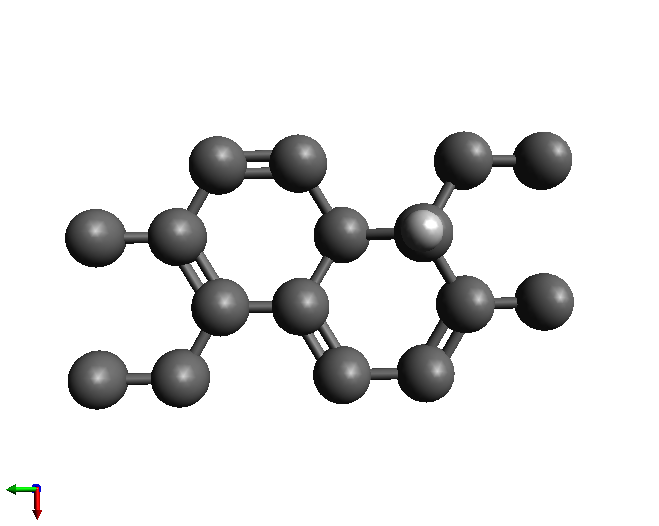
\includegraphics[width=0.4\tw]{./figuras/c16h2_row_close_optimized/c16h2_row_close_optimized1.png}
		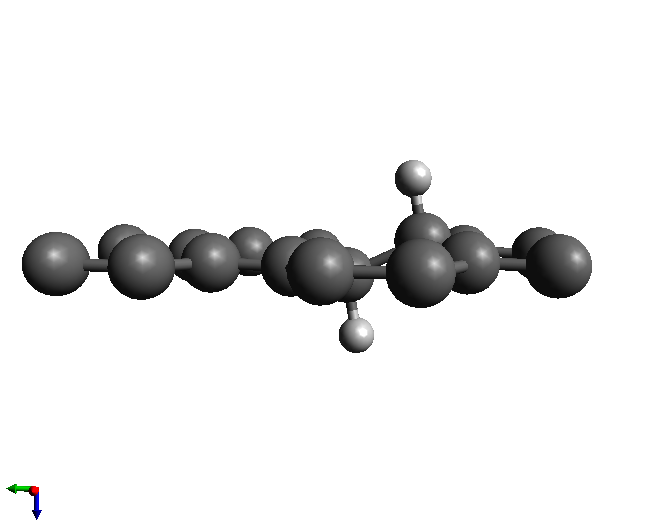
\includegraphics[width=0.4\tw]{./figuras/c16h2_row_close_optimized/c16h2_row_close_optimized2.png}
	\end{center}
	\caption{Estructura C$_{16}$H$_{2}$--row--close desde dos \'angulos de vista.}
	\label{fig:row_struct}
\end{figure}


\begin{figure}[]
	\begin{center}
		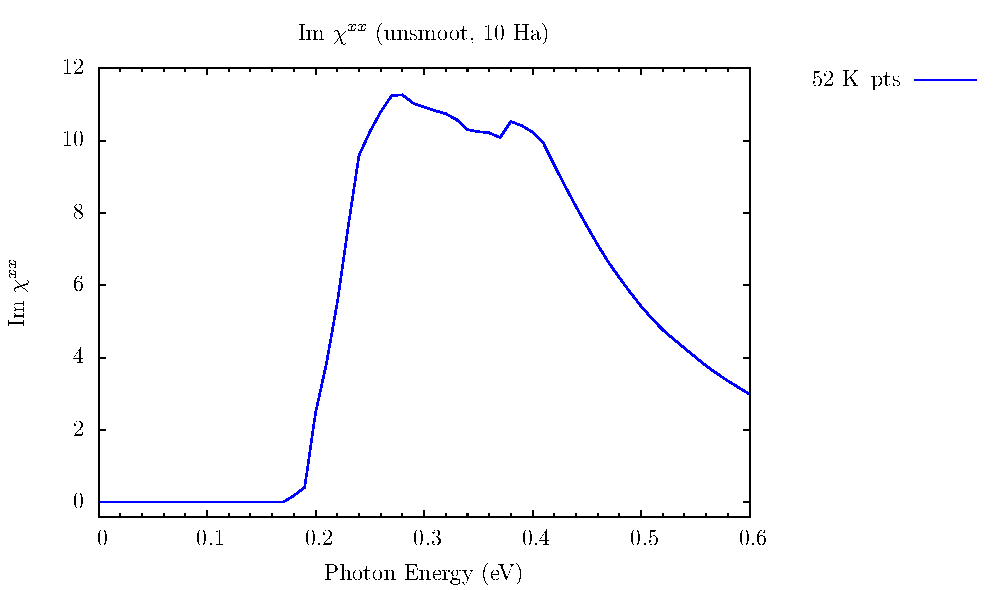
\includegraphics[width=0.8\tw]{./figuras/c16h2_row_close_optimized/res1_chiIm_1_kk_gap.pdf}
	\end{center}
	\caption{An\'alisis del gap para la estructura C$_{16}$H$_{2}$--row--close.}
	\label{fig:row_chi_im_gap}
\end{figure}

\begin{figure}[]
	\begin{center}
		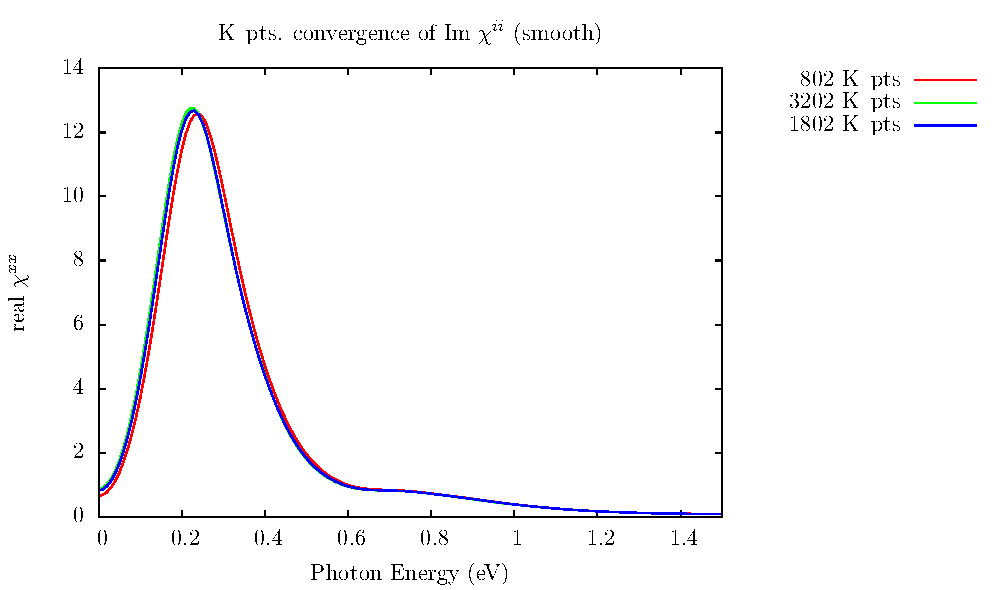
\includegraphics[width=0.7\tw]{./figuras/c16h2_row_close_optimized/res1_Imchi_1_sm.pdf}\\
		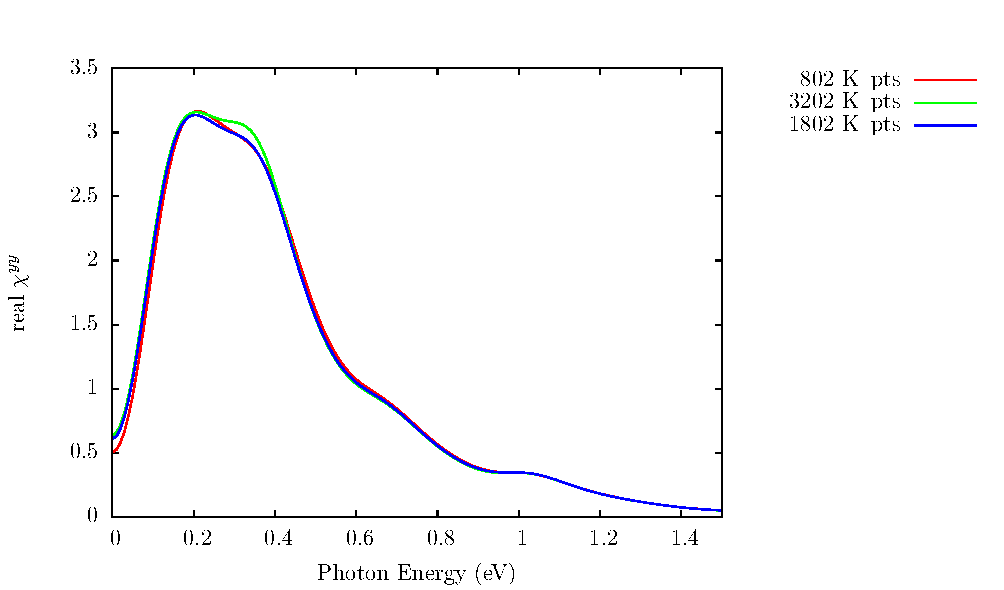
\includegraphics[width=0.7\tw]{./figuras/c16h2_row_close_optimized/res1_Imchi_2_sm.pdf}\\
		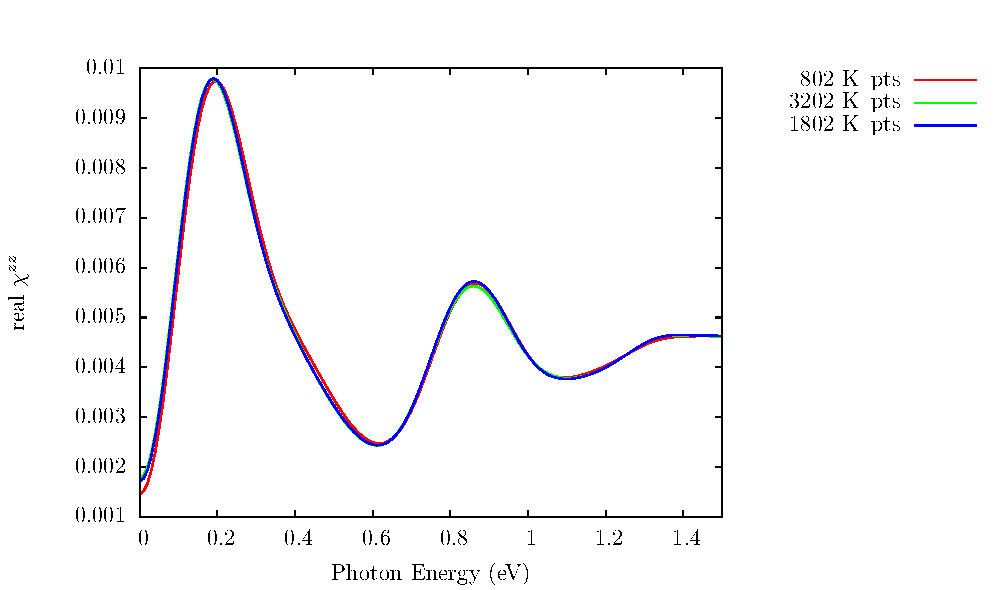
\includegraphics[width=0.7\tw]{./figuras/c16h2_row_close_optimized/res1_Imchi_3_sm.pdf}
	\end{center}
	\caption{Convergencia en puntos \vk \ para la respuesta lineal imaginaria  de la estructura C$_{16}$H$_{16}$--boat.}
	\label{fig:row_Imchi}
\end{figure}

\begin{figure}[]
	\begin{center}
		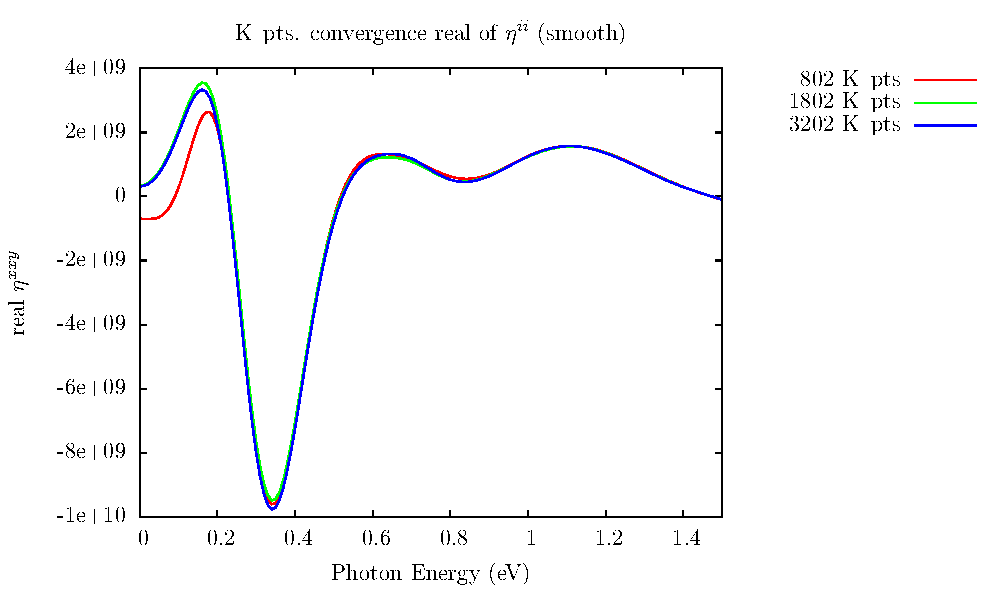
\includegraphics[width=0.7\tw]{./figuras/c16h2_row_close_optimized/res3_eta2_1_sm.pdf}\\
		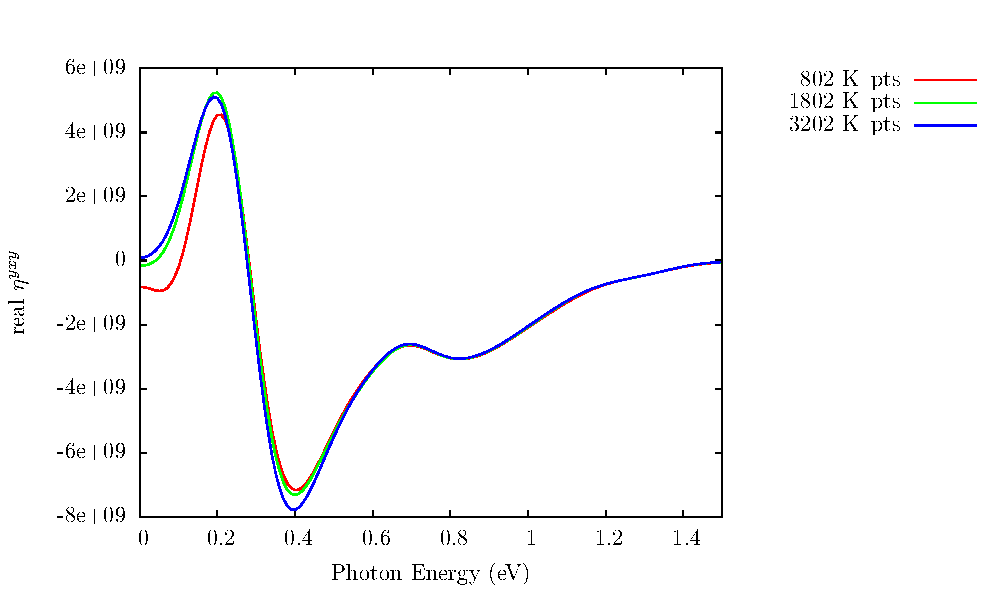
\includegraphics[width=0.7\tw]{./figuras/c16h2_row_close_optimized/res3_eta2_2_sm.pdf}\\
		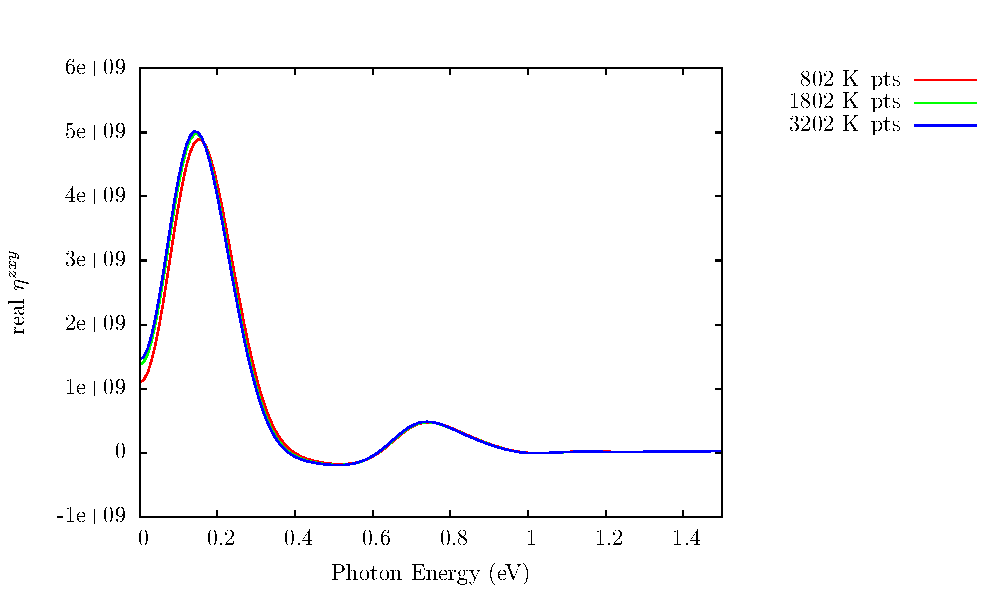
\includegraphics[width=0.7\tw]{./figuras/c16h2_row_close_optimized/res3_eta2_3_sm.pdf}
	\end{center}
	\caption{Convergencia en puntos \vk \ para la inyecci\'on de corriemte  de la estructura C$_{16}$H$_{16}$--boat.}
	\label{fig:row_eta}
\end{figure}

\begin{figure}[]
	\begin{center}
		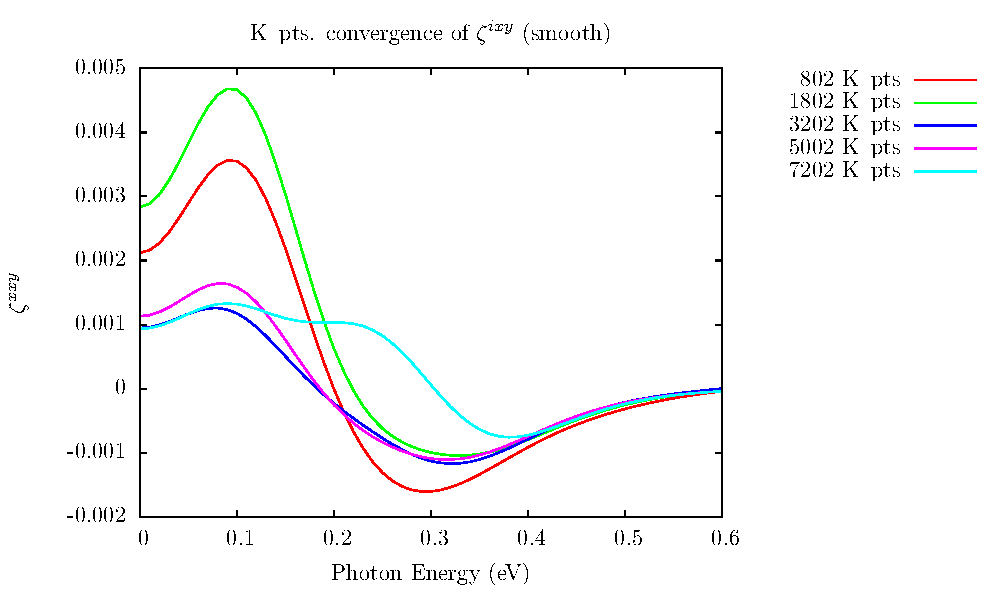
\includegraphics[width=0.7\tw]{./figuras/c16h2_row_close_optimized/res41_zeta_1_sm.pdf}\\
		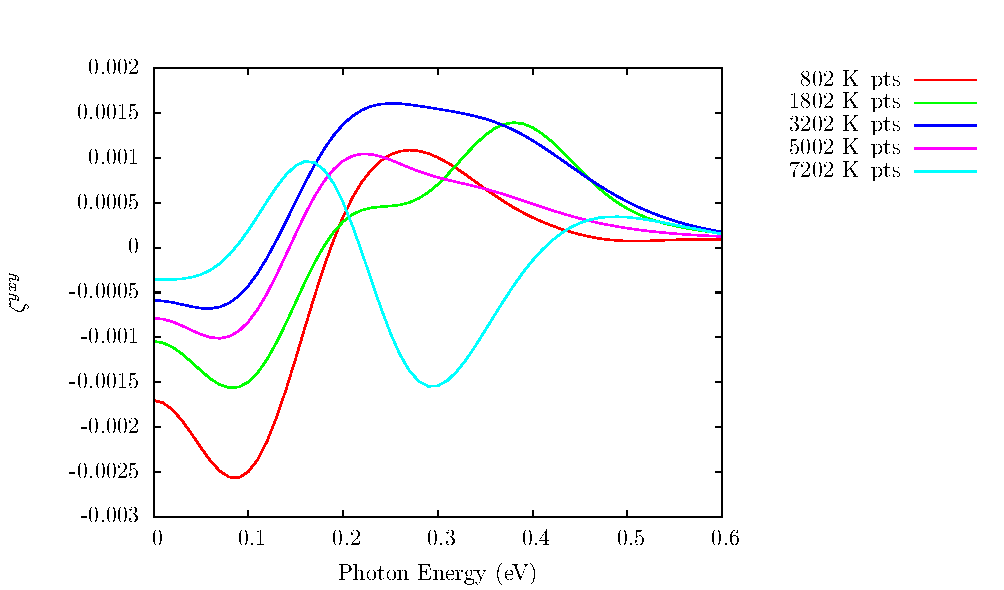
\includegraphics[width=0.7\tw]{./figuras/c16h2_row_close_optimized/res41_zeta_2_sm.pdf}\\
		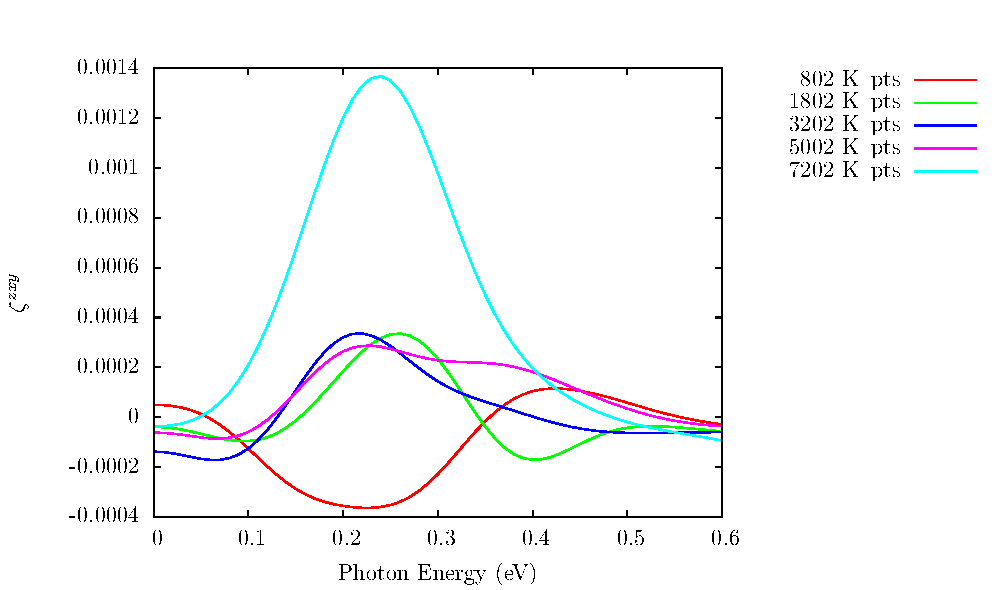
\includegraphics[width=0.7\tw]{./figuras/c16h2_row_close_optimized/res41_zeta_3_sm.pdf}
	\end{center}
	\caption{Convergencia en puntos \vk \ para la inyecci\'on de spin  de la estructura C$_{16}$H$_{16}$--boat.}
	\label{fig:row_zeta}
\end{figure}

\newpage

\section{Estructura C$_{16}$H$_{8}$--alt}\label{section:alt}

En la (Fig. \ref{fig:alt_struct}) se muestran dos \'angulos de vista para esta estructura. Esta es con la primer estructura con la que comenc\'e a trabajar. Para esta estructura se tienen resultados tanto de convergencia para puntos \vk \ (14452 puntos) como para energ\'ia de corte (65\,Ha). A continuaci\'on se muestran los resultados finales par la respuesta lineal imaginaria Im[$\chi$] (Fig. \ref{fig:alt_Imchi}), la inyecci\'on  de corriente $\eta$ (Fig. \ref{fig:alt_eta}) y la polarizaci\'on  de spin $\zeta$ (Fig. \ref{fig:alt_zeta})

\begin{figure}[h!]
	\begin{center}
		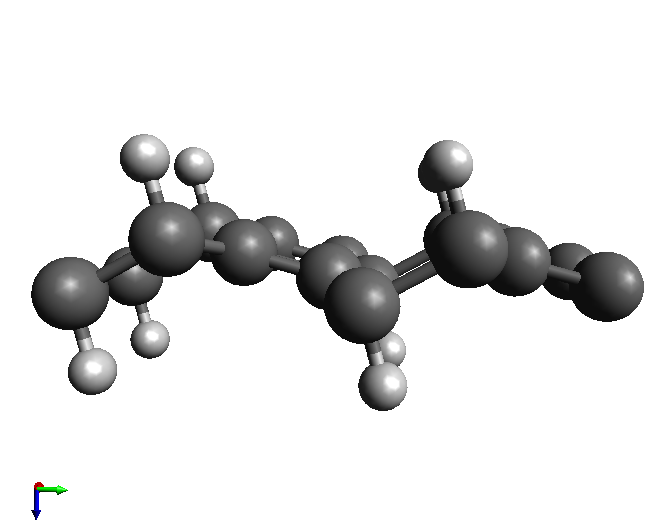
\includegraphics[width=0.4\tw]{./figuras/c16h8_alt/c16h8_alt1.png}
		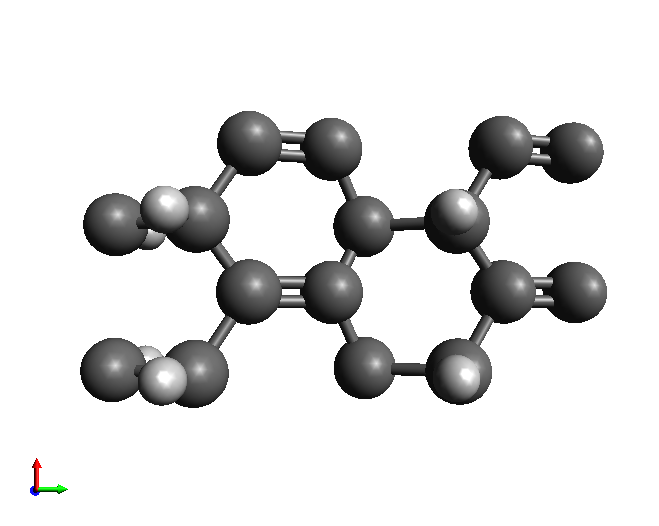
\includegraphics[width=0.4\tw]{./figuras/c16h8_alt/c16h8_alt2.png}
	\end{center}
	\caption{Estructura C$_{16}$H$_{8}$--alt desde dos \'angulos de vista.}
	\label{fig:alt_struct}
\end{figure}


\begin{figure}[]
	\begin{center}
		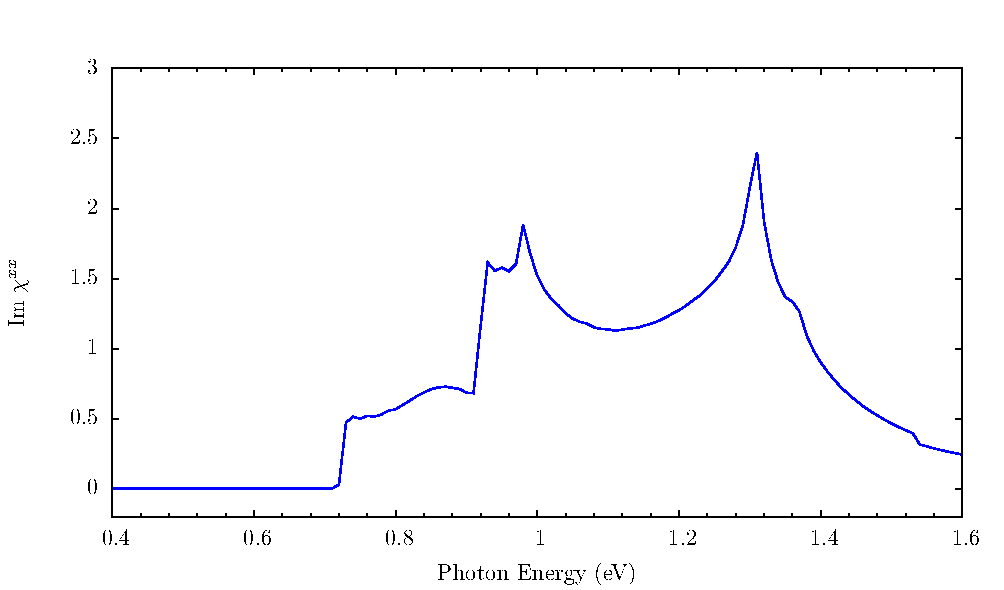
\includegraphics[width=0.7\tw]{./figuras/c16h8_alt/res1_chiIm_1_sm.pdf}\\
		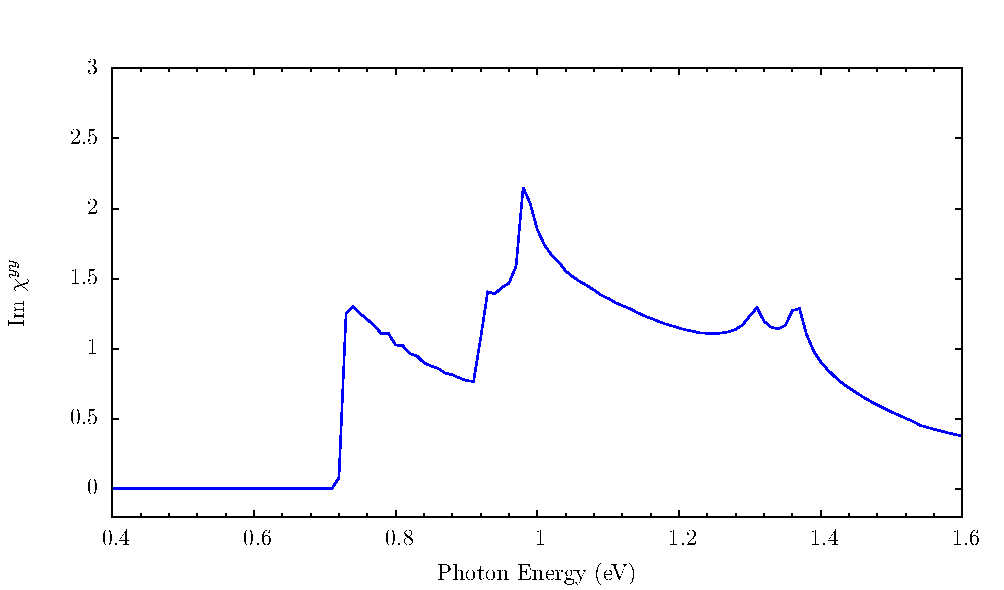
\includegraphics[width=0.7\tw]{./figuras/c16h8_alt/res1_chiIm_2_sm.pdf}\\
		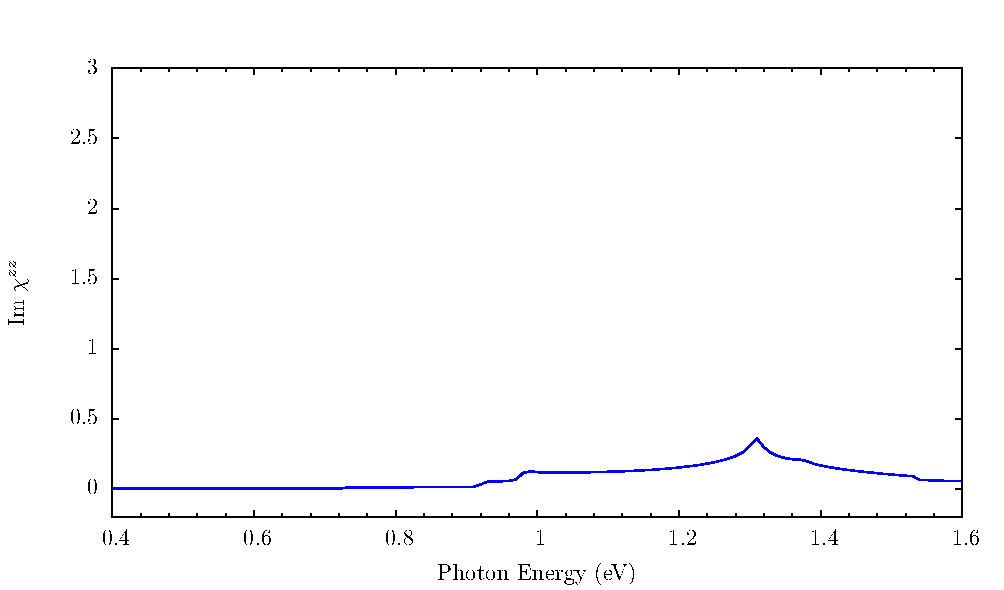
\includegraphics[width=0.7\tw]{./figuras/c16h8_alt/res1_chiIm_3_sm.pdf}
	\end{center}
	\caption{Respuesta lineal imaginaria  de la estructura C$_{16}$H$_{8}$--alt.}
	\label{fig:alt_Imchi}
\end{figure}

\begin{figure}[]
	\begin{center}
		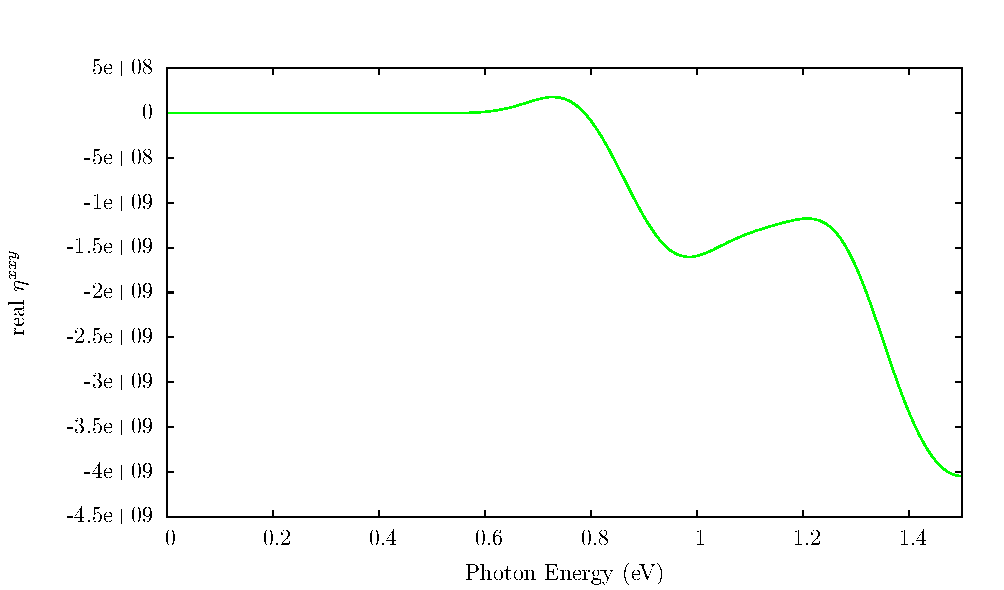
\includegraphics[width=0.7\tw]{./figuras/c16h8_alt/res3_eta2_1_sm.pdf}\\
		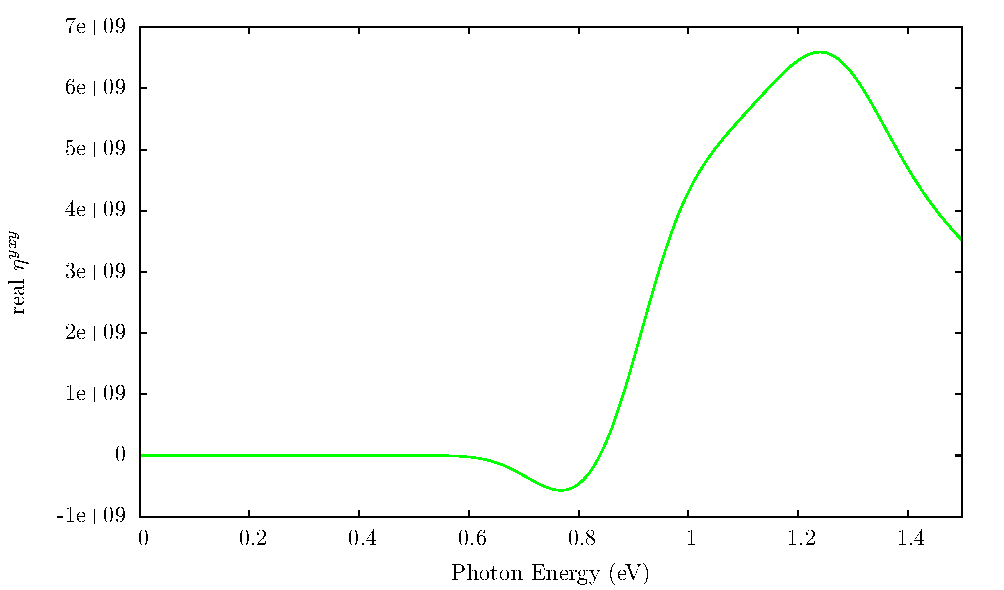
\includegraphics[width=0.7\tw]{./figuras/c16h8_alt/res3_eta2_2_sm.pdf}\\
		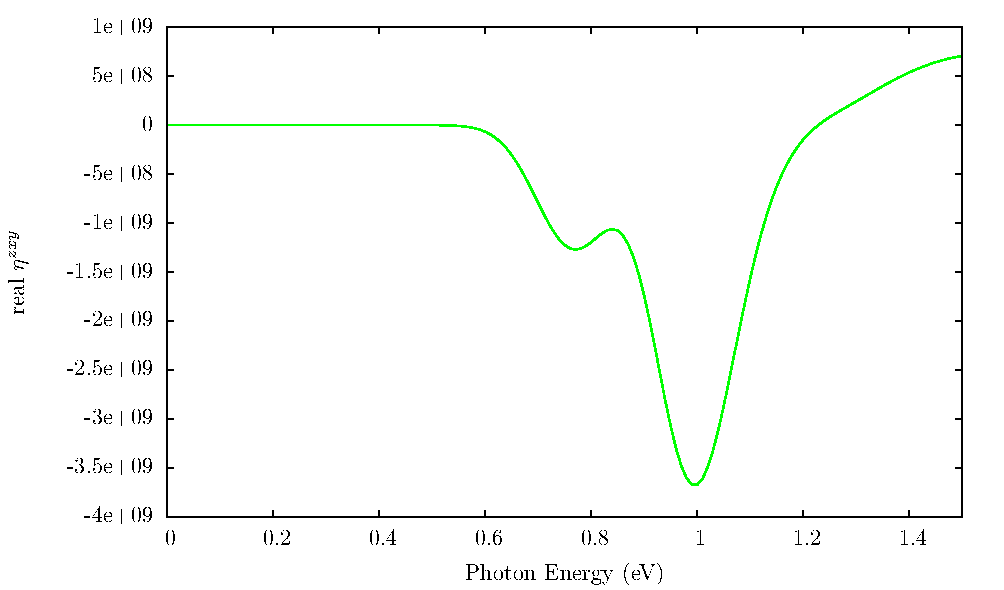
\includegraphics[width=0.7\tw]{./figuras/c16h8_alt/res3_eta2_3_sm.pdf}
	\end{center}
	\caption{Inyecci\'on de corriemte  de la estructura C$_{16}$H$_{8}$--alt.}
	\label{fig:alt_eta}
\end{figure}

\begin{figure}[]
	\begin{center}
		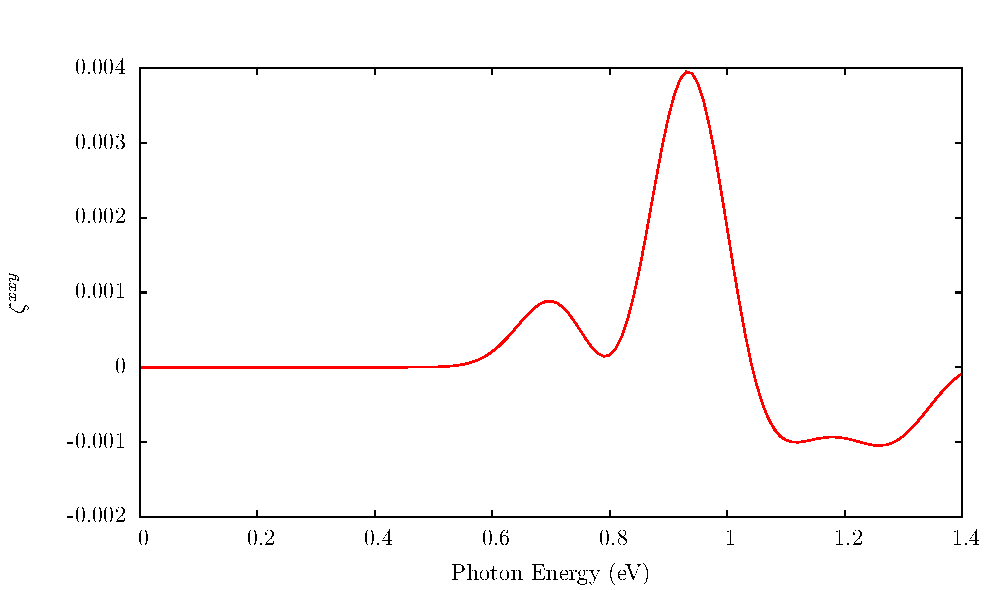
\includegraphics[width=0.7\tw]{./figuras/c16h8_alt/res41z_eta_1_sm.pdf}\\
		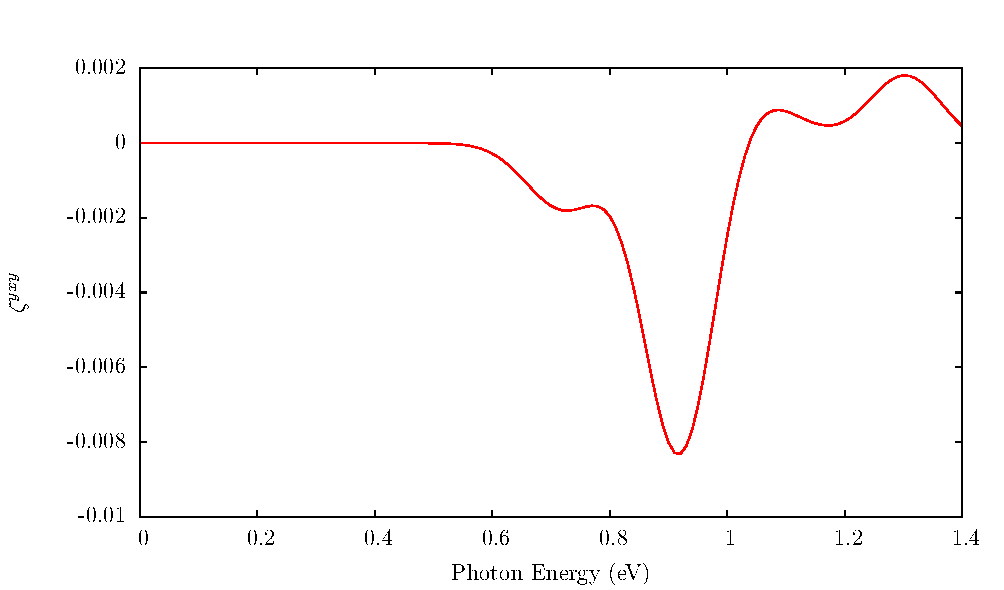
\includegraphics[width=0.7\tw]{./figuras/c16h8_alt/res41z_eta_2_sm.pdf}\\
		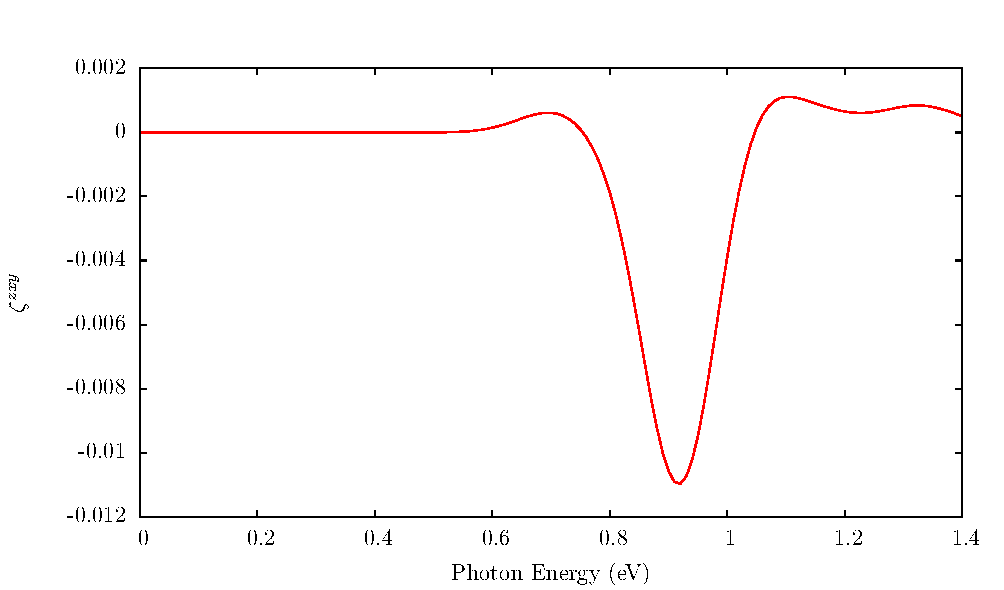
\includegraphics[width=0.7\tw]{./figuras/c16h8_alt/res41z_eta_3_sm.pdf}
	\end{center}
	\caption{Inyecci\'on de spin  de la estructura C$_{16}$H$_{8}$--alt.}
	\label{fig:alt_zeta}
\end{figure}



De la figura (Fig. \ref{fig:alt_Imchi}) se puede ver que el gap LDA es aproximadamente 0.7\,eV.


\newpage

\section{Estructura C$_{16}$H$_{8}$--up}\label{section:up}

En la (Fig. \ref{fig:up_struct}) se muestran dos \'angulos de vista para esta estructura. Esta es con la primer estructura con la que comenc\'e a trabajar. Para esta estructura se tienen resultados de convergencia para puntos \vk \ para todas las respuestas (Figs. \ref{fig:up_Imchi}--\ref{fig:up_zeta}). Como se puede observar, para esta estructura la convergencia se alcanz\'o con 6052 puntos \vk, una cantidad significativamente menor a la necesaria para las estructuras de las secciones \ref{section:row} (Fig. \ref{fig:row_zeta}), \ref{section:alt} y \ref{section:boat}.

De la (Fig. \ref{fig:up_Imchi}) se puede ver que el gap LDA para esta estructura es 0.38\,eV. 

\begin{figure}[h!]
	\begin{center}
		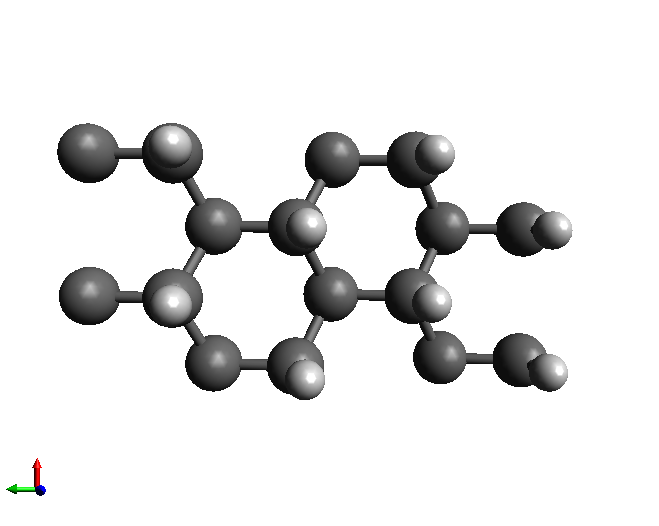
\includegraphics[width=0.4\tw]{./figuras/c16h8_up/c16h8_up-structure1.png}
		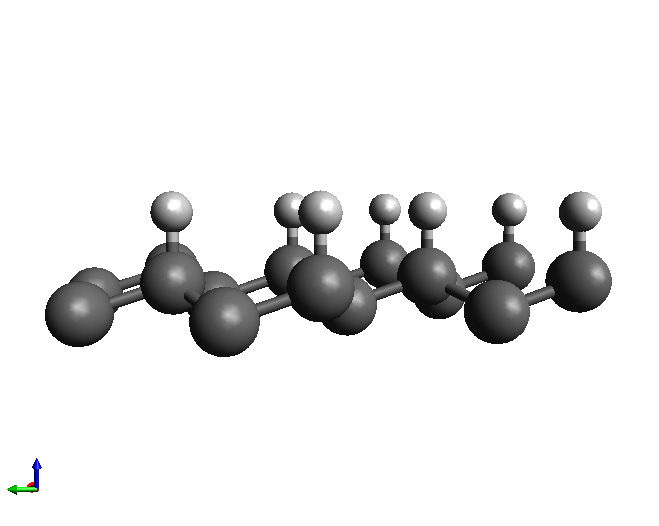
\includegraphics[width=0.4\tw]{./figuras/c16h8_up/c16h8_up-structure2.png}
	\end{center}
	\caption{Estructura C$_{16}$H$_{8}$--up desde dos \'angulos de vista.}
	\label{fig:up_struct}
\end{figure}


\begin{figure}[]
	\begin{center}
		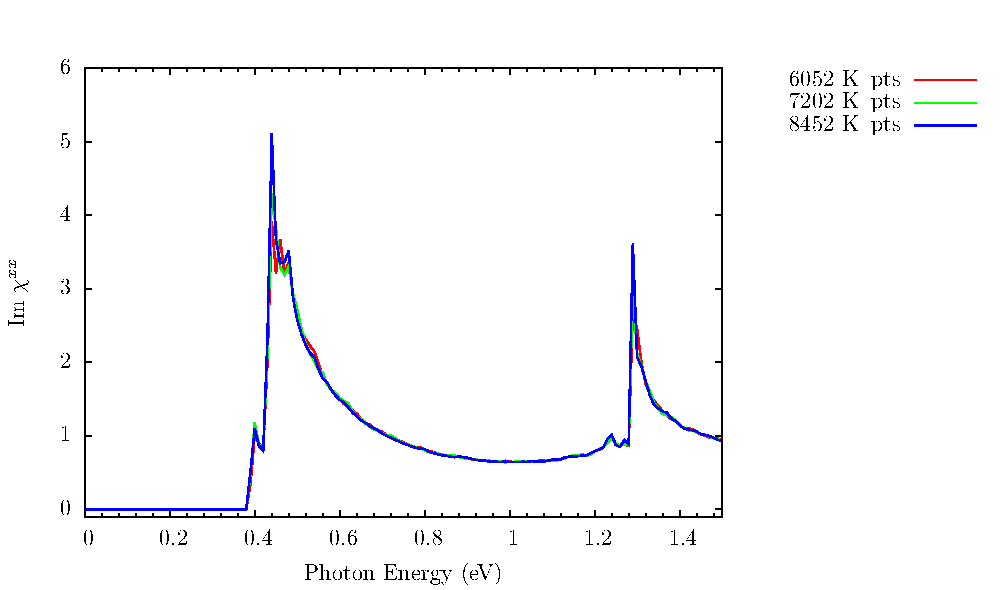
\includegraphics[width=0.7\tw]{./figuras/c16h8_up/res1_chiIm_1_sm.pdf}\\
		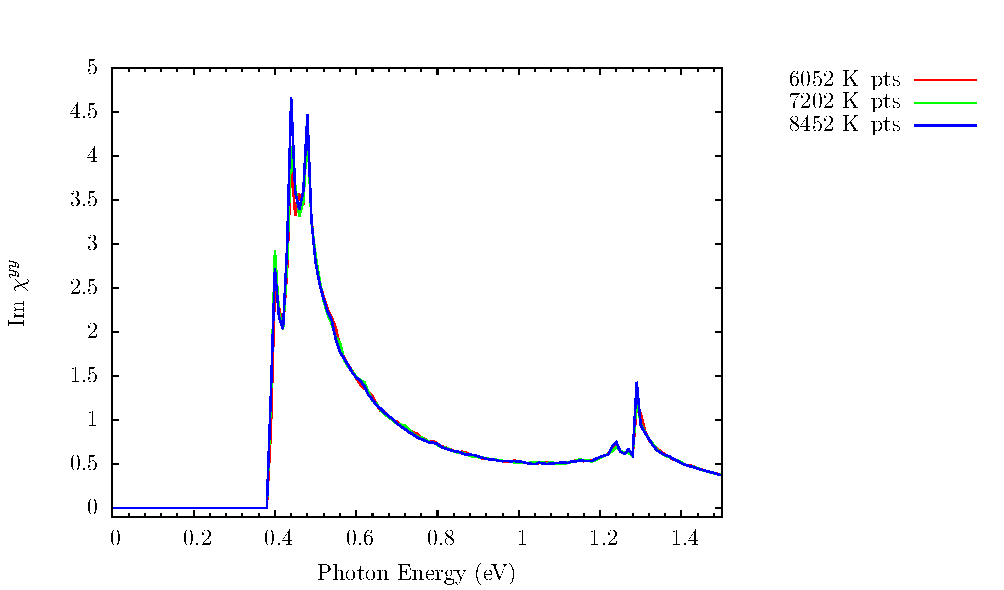
\includegraphics[width=0.7\tw]{./figuras/c16h8_up/res1_chiIm_2_sm.pdf}\\
		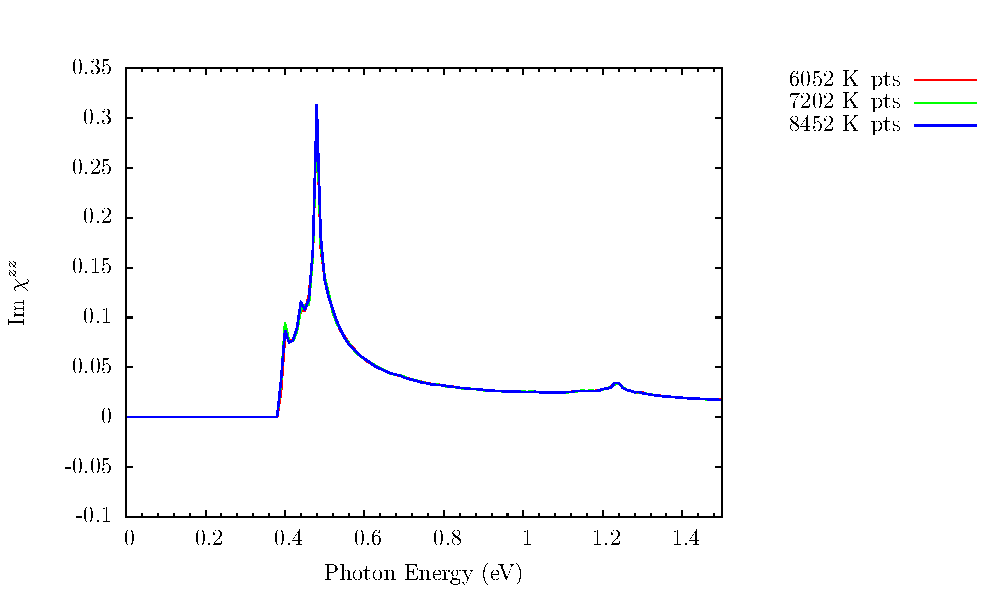
\includegraphics[width=0.7\tw]{./figuras/c16h8_up/res1_chiIm_3_sm.pdf}
	\end{center}
	\caption{Convergencia  en puntos \vk \ para la respuesta lineal imaginaria  de la estructura C$_{16}$H$_{8}$--up (sin suavizado).}
	\label{fig:up_Imchi}
\end{figure}

\begin{figure}[]
	\begin{center}
		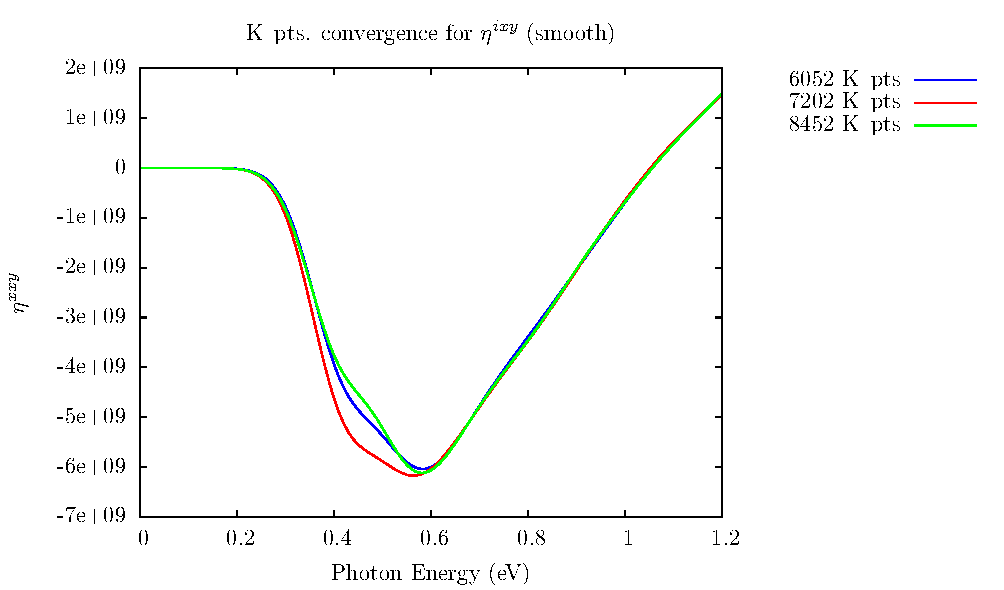
\includegraphics[width=0.7\tw]{./figuras/c16h8_up/res3_eta_1_sm.pdf}\\
		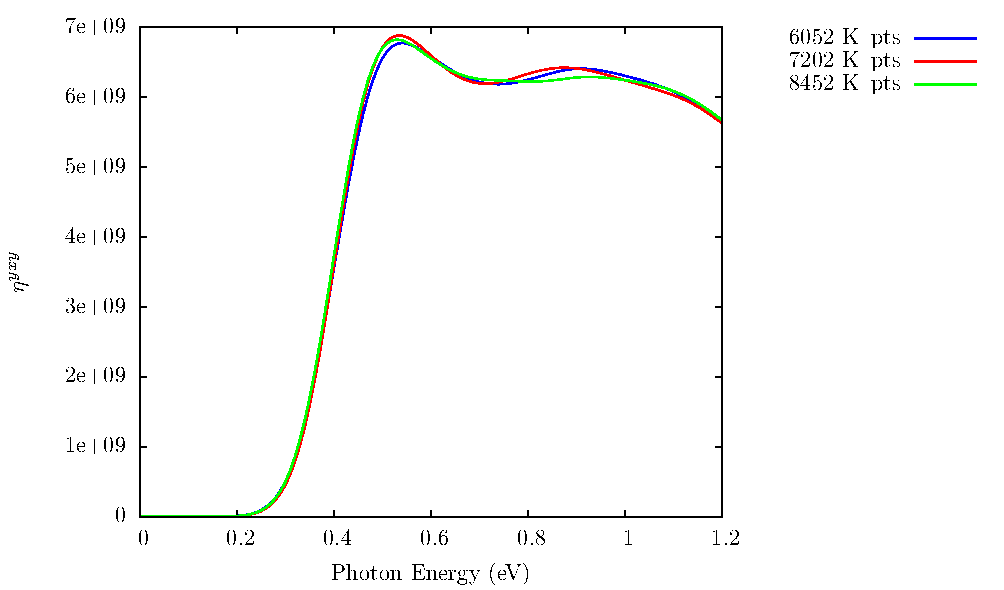
\includegraphics[width=0.7\tw]{./figuras/c16h8_up/res3_eta_2_sm.pdf}\\
		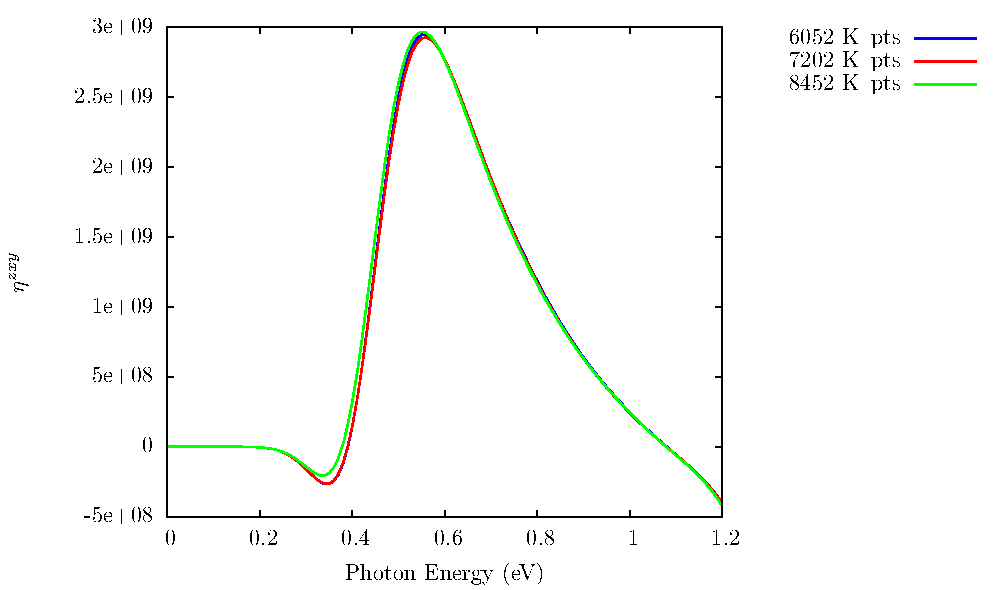
\includegraphics[width=0.7\tw]{./figuras/c16h8_up/res3_eta_3_sm.pdf}
	\end{center}
	\caption{Convergencia en puntos \vk \ para la inyecci\'on de corriemte  de la estructura C$_{16}$H$_{8}$--up.}
	\label{fig:up_eta}
\end{figure}

\begin{figure}[]
	\begin{center}
		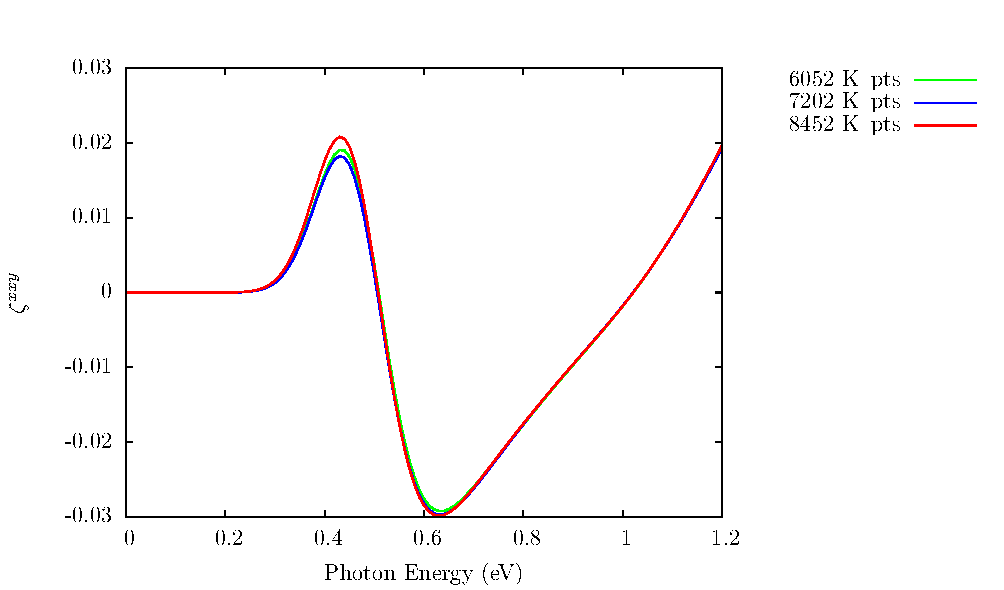
\includegraphics[width=0.7\tw]{./figuras/c16h8_up/res41_zeta_1_sm.pdf}\\
		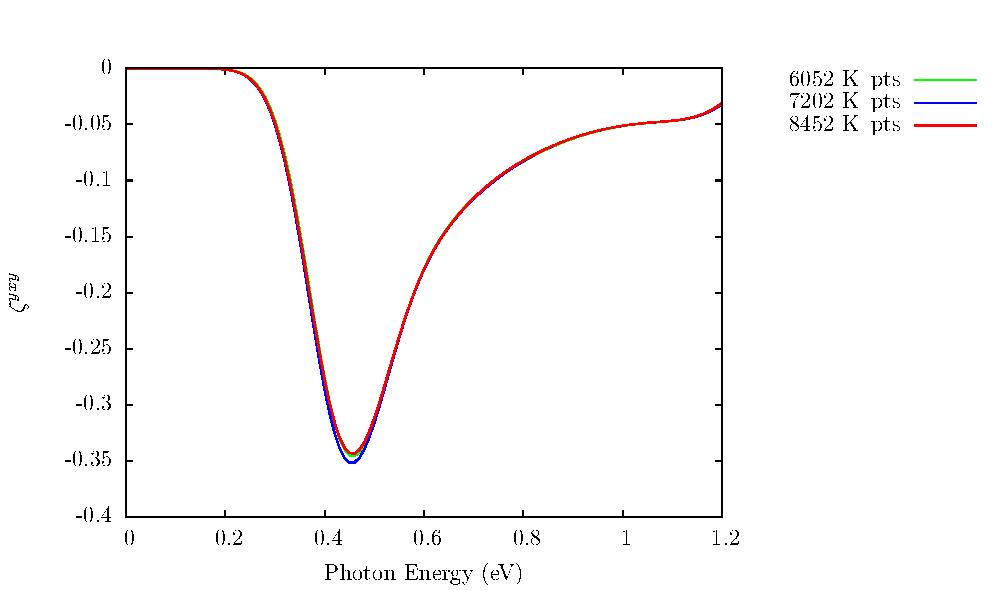
\includegraphics[width=0.7\tw]{./figuras/c16h8_up/res41_zeta_2_sm.pdf}\\
		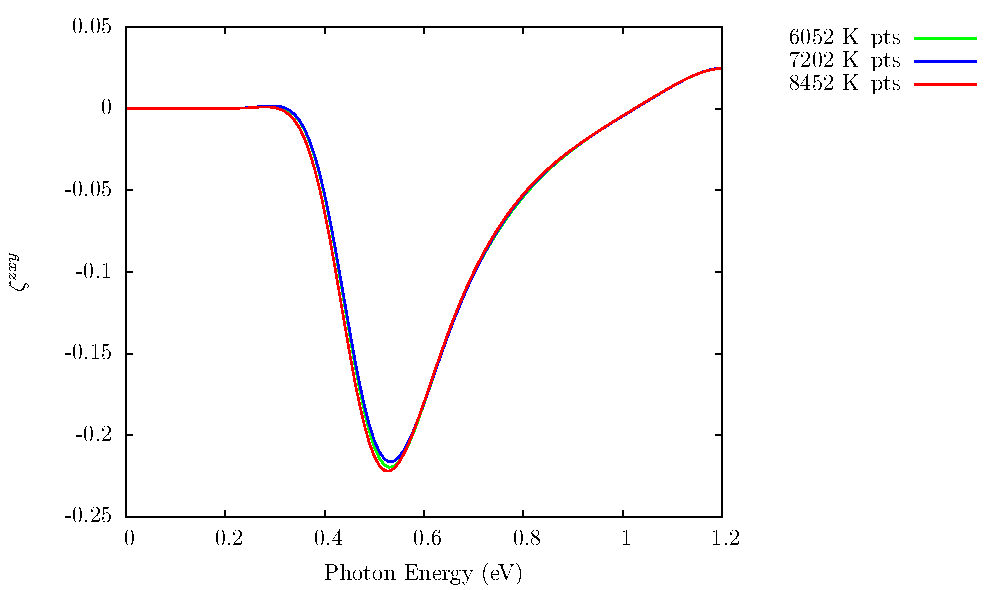
\includegraphics[width=0.7\tw]{./figuras/c16h8_up/res41_zeta_3_sm.pdf}
	\end{center}
	\caption{Convergencia en puntos \vk \ para la inyecci\'on de spin  de la estructura C$_{16}$H$_{8}$--up.}
	\label{fig:up_zeta}
\end{figure}

\newpage

\section{Estructura C$_{16}$H$_{16}$--boat}\label{section:boat}

En la (Fig. \ref{fig:boat_struct}) se muestran dos \'angulos de vista para esta estructura. Esta es con la estructura a la que m\'as teimpo le he dedicado y en la que no se ha llegado a la convergencia en puntos k. La (Fig. \ref{fig:boat_chi_im_gap}) muestra un rango reducido de Im[$\chi^{xx}$] (sin suavizado) para una energ\'ia de 10\,Ha y s\'olo 53 puntos \vk. De all\'i se puede ver que el gap LDA es aproximadamente 0.17\,eV. 

La (Fig. \ref{fig:boat_chi_im_gap}) muestra un rango reducido de Im[$\chi^{xx}$] (sin suavizado) para una energ\'ia de 10\,Ha y tres valores distintos de puntos \vk. De all\'i se puede ver que el gap LDA es aproximadamente 0.2\,eV.

De esta estructura es de la que te he enviado los \'ultimos reportes, incluyendo las respuestas con medios integrandos. Se tiene convergencia para todas las respuestas, exceptuando par el tenson $\zeta^{abc}$.

Antes de correr con una red desplazada de puntos me comunico contigo par ponernos de acuerdo acerca de si lo estoy haciendo bien, o bien, como t\'u sugeriste, descartarla.


\begin{figure}[h!]
	\begin{center}
		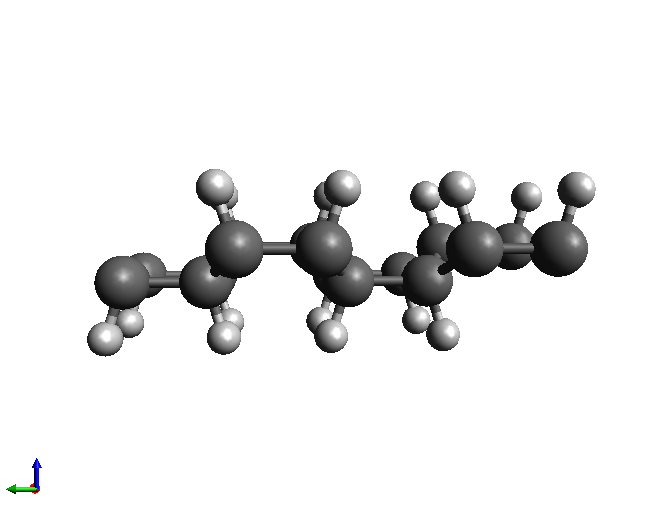
\includegraphics[width=0.4\tw]{./figuras/c16h16_boat/c16h16-boat-structure1.png}
		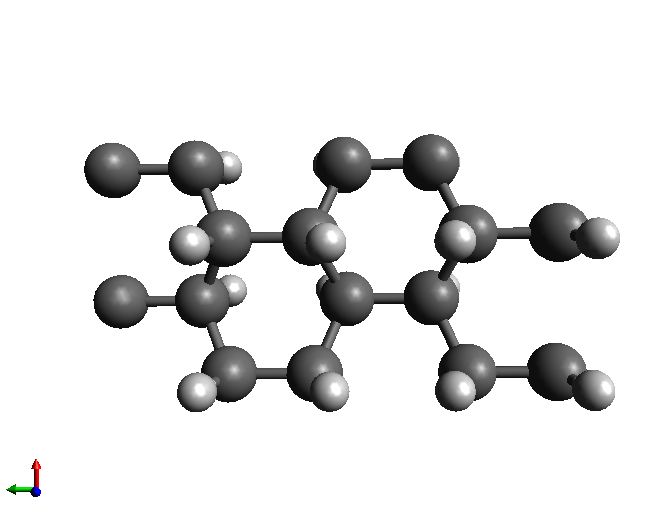
\includegraphics[width=0.4\tw]{./figuras/c16h16_boat/c16h16-boat-structure2.png}
	\end{center}
	\caption{Estructura C$_{16}$H$_{16}$--boat desde dos \'angulos de vista.}
	\label{fig:boat_struct}
\end{figure}


\begin{figure}[]
	\begin{center}
		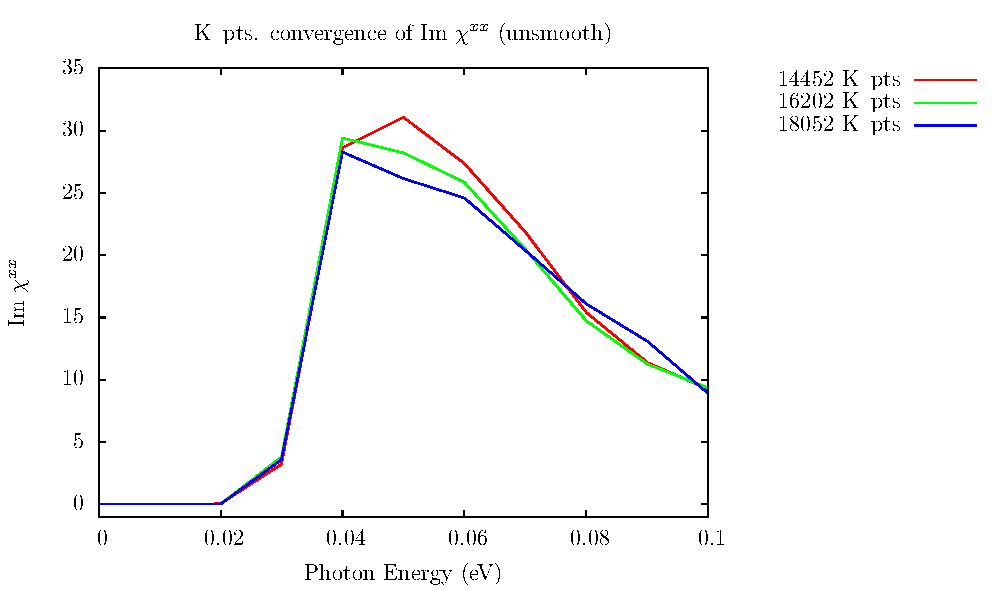
\includegraphics[width=0.7\tw]{./figuras/c16h16_boat/res1_chiIm_1_sm_gap.pdf}
	\end{center}
	\caption{An\'alisis del gap para la estructura C$_{16}$H$_{16}$--boat.}
	\label{fig:boat_chi_im_gap}
\end{figure}

\newpage

\section{Estructura C$_{16}$H$_{16}$--chair}\label{section:chair}

En la (Fig. \ref{fig:chair_struct}) se muestran dos \'angulos de vista para esta estructura. Esta es una de las estructuras usadas en la tesis de maestr\'ia. Como te mencin\'e anteriormetne, los c\'alculos son incorrectos. Estoy esperando a terminar con las dem\'as estructuras par comenzar a trabajar con esta.

\begin{figure}[]
	\begin{center}
		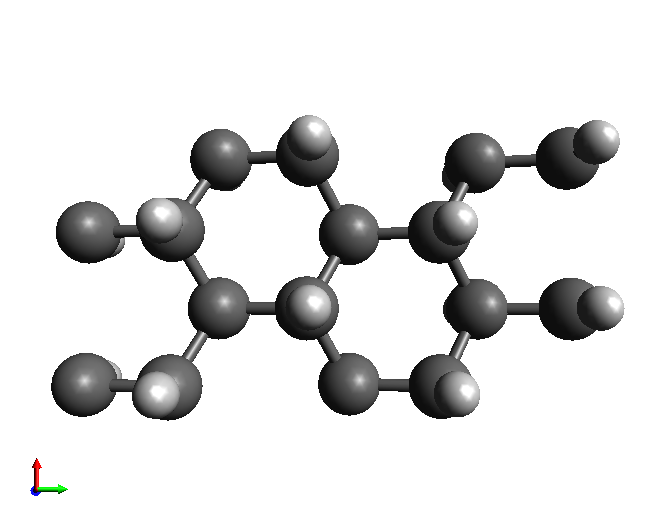
\includegraphics[width=0.4\tw]{./figuras/c16h16_chair/C16H16_chair1.png}
		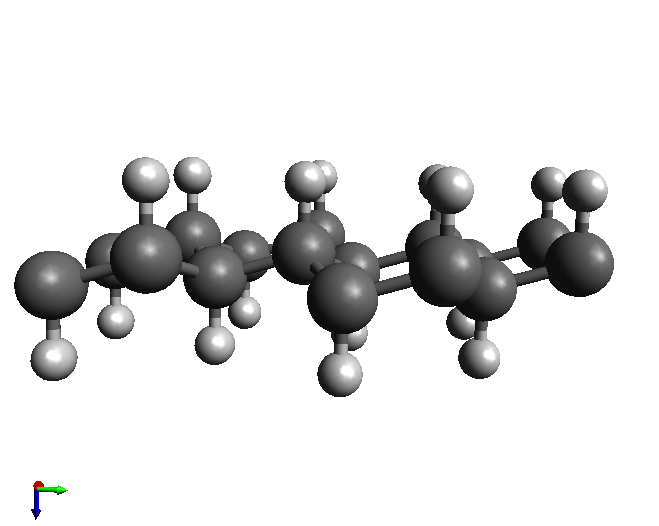
\includegraphics[width=0.4\tw]{./figuras/c16h16_chair/C16H16_chair2.png}
	\end{center}
	\caption{Estructura C$_{16}$H$_{16}$--boat desde dos \'angulos de vista.}
	\label{fig:chair_struct}
\end{figure}


\end{document}

